%!TEX root = ../../dissertation.tex
%%%%%%%%%%%%%%%%%%%%%%%%%%%%%%%%%%%%%%%%%%%%%%%%%%%%%%%%%%%%%%%%%%%%%%%%%%%%%%%%
\section{Measurements}
\label{c3:measurements}

With these playback models at hand, this section demonstrates how to conduct actual evaluations of reliable streaming protocols with it.

As discussed, there are numerous incarnations of reliable streaming protocols in use. Almost all of them follow the same basic approach but with slight variations in execution and choice of playback strategies and corresponding parameters. But it is exactly these choices that can have a large impact on the streaming process and resulting quality. 

The problem lies in comparing these protocols to each other. Each of them is usually tied to a specific -- and most often proprietary closed source -- streaming player. Setting up all these players in one testbed is a huge effort and requires very specific software environments to be used on the client machines. Moreover, these players are built with user interaction and not automation and directly measuring the outcome in mind. This can still be achieved through extensive workarounds, but must be tailored to every player application. The presented approach avoids this hassle and provides a concise way to test any conceivable playback strategy in one single test setup.


%%
\subsection{Progressive Streaming Measurement Framework}

To enable quick evaluations for progressive streaming the framework follows a two phase approach, separating the active online recording phase from the passive playback emulation. Recording data is very time intensive and cannot be sped up when conducting investigation of a real world process, and not relying on simulated data. It still replicates the steps a user would perform to consume a media stream on a playback device. Through appropriate configuration different scenarios can be modeled, e.g. network conditions, behavior and specifics of the user device.
 
\begin{figure}[htb]
    \includegraphics[width=\textwidth]{images/measurement-model.pdf}
    \caption{Measurement framework for progressive streaming playback strategies overview.}
    \label{c3:fig:framework}
\end{figure}

Figure \ref{c3:fig:framework} depicts the framework for a streaming evaluation testbed. In phase one the stream's transmission is conducted and recorded on a per-packet level. Stream data is transmitted to the client from a server which can be any actual streaming service on the Internet or a local server under the testbed's control, eliminating undesired side effects caused by the Internet connection. 

The traffic is directed through a network emulation node capable of altering the network \gls{QoS} parameters, i.e. latency, jitter, and packet loss. The parameters can be set according to stochastic models derived from actual network architectures. Instead of network emulation, any preexisting architecture can also be placed here to achieve more accurate results for the intended target. This is especially helpful for complex infrastructures hard to model or with no good and concise models available yet, for example mobile and mobile core networks with the influence of encapsulating traffic into bearers.

The measurement host downloads and records the video stream as a network trace. For progressive \gls{HTTP} streaming, a single request on the video file is issued and the \gls{TCP} connection maintained until the file has fully arrived.
This process is recorded as basis for the second phase. These traces should consist of the size and timestamp of every incoming packet. More detailed traces can be used to scrutinize other layers of the connection, e.g. the dynamics of TCP receive window size. Additionally the received file is decoded yielding a trace of all video frame sizes and playout timestamps.

In the second pass, these two traces are then used to feed the actual reliable streaming playback model described before. This conducted by a closed-loop emulation process calculating the current buffer fill level based on the collected transmission and video frame traces for every point in time. 

All of the progressive streaming -- i.e. non-adaptive -- strategies can be tested on the same trace set.
In simple \gls{HTTP} streaming, the transmission is not controlled by the streaming application and no rate control is conducted. Therefore, recording the packet trace and simulating playback are completely decoupled, as the latter cannot influence the former.  This enables fast and efficient comparison of non-feedback protocols subject to the same network conditions.

The emulator then generates playback stalling statistics, specifically their number and duration, to compare the effect of the different strategies on the same trace. With these results, parameter settings for playback strategies can also be iteratively tested and improved leading to an empirical calibration of playback strategies instead of relying on best practices.

One of the drawbacks of this model-based emulation approach is of course the reliance on suitable models and playback strategies for the stream protocols under scrutiny. Obtaining these from proprietary streaming clients, can be a difficult reverse-engineering process.


%%
\subsection{Adaptive Streaming Measurement Framework}

Up to this point, the measurement framework is only suitable for progressive streaming omitting any adaptive strategy. This second framework modifies this and additionally allows for the testing of adaptive playback strategies. However, to achieve this, the advantageous two phase setup cannot be employed anymore.

\begin{figure}[htb]
    \includegraphics[width=\textwidth]{images/feedback-measurement-model.pdf}
    \caption{Measurement framework for adaptive streaming playback strategies overview.}
    \label{c3:fig:framework-feedback}
\end{figure}

Figure~\ref{c3:fig:framework-feedback} shows the adapted framework. The playback emulation process is now directly fed with the stream transmission without recording it first. The emulation is now an online process and has to be conducted in realtime. This enables the emulator to react on the current streaming state and request an alteration from the server. The adaptation spectrum ranges from the timing of stream segment retrieval to the chosen quality level of future segments. 

While allow for a wider range of playback strategies, this approach is also inherently slower as it does not allow a speed-up beyond realtime, limiting its usability somewhat. Therefore, a transition to a full simulative approach is suggested. This is path is further explored and discussed in Section~\ref{c5:mobilestreamingtestbed}.

\todo{check simulation approach ref or further explain simulation}


%%
\subsection{Technical Implementation}

To conduct measurements, the described two phase progressive streaming measurement framework was implemented in a testbed. This testbed consists of three interconnected physical nodes running Linux. 

The optional streaming server houses an Apache httpd\footnote{\url{https://httpd.apache.org/}} Web server, hosting the files that are to be streamed. Alternatively, Internet streaming service traffic can also be directly routed through the network emulation node.

The network emulation node uses the existing \gls{QoS} capabilities of the Linux kernel, dubbed NetEm \cite{hemminger2005network}, to add latency and packet loss to the transmission as well as to act as a bandwidth bottleneck. The additional delay is set deterministically, the loss follows a uniform distribution without any correlation in the transmission.

To both retrieve the streaming file and record the transmission process at the client, curl\footnote{\url{http://curl.haxx.se/}} is used. If so desired, tcpdump\footnote{\url{http://www.tcpdump.org/}} can also be facilitated to achieve a higher recording precision. The video file is then parsed for its frames and sizes using mplayer\footnote{\url{http://www.mplayerhq.hu/}} with libav\footnote{\url{https://libav.org/}}. The traces are then put into the actual playback emulation, implemented by custom Python-based code and statistically evaluated with Python as well as R.



%%
\subsection{Measurement Series and Evaluations with the Framework}
%[visualization and results (does yt still work well with high delay/loss?)]
%[performance evaluation (BWs, played vs received data)]
%Also observed and analyzed. The deduce that the initial buffering time and the later block sending rate are directly correlated. 64kb blocks, probably due to GFS, problems with this method, ...
%These Quality-of-Service parameters loss and delay do not have any direct influence on the downloading process but instead have negative impacts on the throughput of the underlying TCP due to its congestion control feature and, in the end, serve as another source of delay and jitter.

This implementation has been used to conduct a comparative study of two theoretical and two real world playback strategies. They are tested for their susceptibility to worsening network \gls{QoS}, latency and loss in this case.

The video used in the experiment was streamed from the YouTube web site providing a realistic foundation for the experiments. This also enables a server side pacing mechanism adjusted to the video bitrate for free
Details on the video used in the experiment are available in Table~\ref{c3:tbl:videoparams}. Two measurement series are performed with this video, both only differ in the network emulator setting. The first series increasingly adds packet loss to the stream, with the second series altering the packet delay. 

\begin{table}[htbp]
    \centering
    \caption{Test Video Parameters}
    \label{c3:tbl:videoparams}
    \begin{tabu}{|l|X[r]|}
        \hline
        Parameter & Value \\ \hline
        Video Duration  & \SI{92.536}{\second}\\
        Size & \SI{9.61}{\mebi\byte} \\
        Framerate & \SI{23.976}{\per\second} \\
        Average Video Bitrate & \SI{871}{\kilo\bit\per\second} \\
        Codecs & AVC+AAC \\ \hline
    \end{tabu}
\end{table}


%% latency
In the latency measurement series, the emulator delayed forwarding the packets for a constant amount of time
The latency was increased in \SI{100}{\milli\second} steps, up to a total of \SI{5000}{\milli\second}. The added latency is split up evenly between the uplink and the downlink.


It can be stated, that all playback strategies will generally work very similar under good network conditions. If sufficient bandwidth is available, they will play videos with almost no delay or intermediate buffering. 
If, however, the achievable \gls{TCP} goodput is close to the average video bitrate, the buffer can be quickly drained by short deviations from the average transmission and video bit rates. The \gls{TCP} goodput can be limited by high latency and loss. Many \gls{TCP} congestion control algorithms depend on the round trip time. If the \gls{RTT} is high, the congestion window will increase much slower. High latency can also trigger \gls{TCP} timeouts and retransmissions, and in turn decrease the congestion window, further impacting the goodput. 

%% <-- WIP

The latency measurements are depicted in Figures \ref{c3:fig:eval-latency-stallingtime} and \ref{c3:fig:eval-latency-numstalls}. The stalling time increases with the additional latency. The Initial Start Delay model provides the best possible result in terms of pure stalling time. On the other hand, Figure \ref{c3:fig:eval-latency-numstalls} shows the Stalling model provides always the worst result for the number of stalls. Any other model will lie beyond that line. The Flash and HTML5 models both run in just a few buffering events which however tend to increase in length with rising latency. Attributed to the simple and optimistic assumption of the Flash model, stalling time is usually lower than with HTML5, at the cost of slightly more buffering events.
 

\begin{figure}[htb]
    \centering
    \includegraphics[width=\textwidth]{images/eval-latency-stallingtime.pdf}
    \caption{Total stalling time.}
    \label{c3:fig:eval-latency-stallingtime}
\end{figure}

\begin{figure}[htb]
    \centering
    \includegraphics[width=\textwidth]{images/eval-latency-frequency.pdf}
    \caption{Playback model observations on additional latency. Number of stalls.}
    \label{c3:fig:eval-latency-numstalls}
\end{figure}


% loss
In the loss experiment series, uncorrelated uniformly distributed loss was added in both the uplink and the downlink direction. The loss was increased in $2\%$ steps up to a total additional loss of $14\%$

TCP goodput is even more severely affected by packet loss. A lost packet results in a duplicate acknowledgement, retransmissions, and a decrease of the congestion window. The problem gets worse if also the ACKs are lost and the connection stalls on missing old segments without which the playback cannot proceed. Figure xyz shows some exemplary measurements for a loss scenario. While additional packet losses of up to four percent seem to have no noticeable impact on streaming quality, the total stalling time suffers a large increase for any model as seen in Fig. \ref{c3:fig:eval-loss-stallingtime} rendering any streaming attempts practically unusable. Figure \ref{c3:fig:eval-loss-numstalls} shows the extremity of the Stalling model compared to other models reaching a number orders of magnitude larger than any other model.
As a result, when planning a network for streaming applications, the maximum loss should be kept below the noticed mark to achieve reasonable streaming quality. 


\begin{figure}[htb]
% used yt-delay/hPUGNCIozp0_delay_100 2, spyder with matplotlib config patch
    \centering
    \includegraphics[width=\textwidth]{images/eval-loss4mb-stallingtime.pdf}
    \caption{Playback model observations on additional packet loss. Total stalling time.}
    \label{c3:fig:eval-loss-stallingtime}
\end{figure}

\begin{figure}[htb]
    \centering
    \includegraphics[width=\textwidth]{images/eval-loss4mb-frequency.pdf}
    \caption{Playback model observations on additional packet loss. Number of stalls.}
    \label{c3:fig:eval-loss-numstalls}
\end{figure}
 
 %%




For this the simple stalling model is used because this results in the shortest possible playback duration in every scenario. Furthermore, we used a network emulation testbed to subject the video streaming to increased loss and latency while fixing the maximum network bandwidth and observe the influence on the QoE.

First use case to show how our system works: Progressive HTTP streaming. Will show adaptability to adaptive streaming and different protocols. For this comparison we used a video of about \SI{90}{second} length and network conditions that could not fulfill the video bitrate in time and hereby forced stalling to occur.

We performed two measurement series, one with increased packet loss, the other one adding latency to the path. For each value of loss and latency a mean total stalling time was calculated out of five separate experiments to eliminate temporal and network load influences. Additionally, standard deviations are shown in the resulting graphs. We clearly notice very large deviations in some experiments. Some of these can be explained by connection timeouts and later resumption of the streaming. Furthermore, an exponential regression line shows the trend of the total stalling times in the experiments.




%% <-- %% end WIP

\begin{figure}[htbp]
    \centering
    \includegraphics[width=\textwidth]{images/R-delayseries.pdf}
    \caption{Total buffering time and linear smooth for degraded network parameter scenarios. Latency Graph.}
    \label{c3:fig:delayseries}
\end{figure}

\begin{figure}[htbp]
    \centering
    \includegraphics[width=\textwidth]{images/R-lossseries.pdf}
    \caption{Total buffering time and linear model for degraded network parameter scenarios. Loss Graph.}
    \label{c3:fig:lossseries}
\end{figure}

Figure \ref{c3:fig:delayseries} displays the results of of the latency measurement series with up to five seconds of additional delay. In the worst case the stalling time increases to about 50 seconds. In mobile scenarios latencies of up to 2 seconds can be expected, which would, according to our measurements, result in a maximum mean stalling time of 15 seconds for a 90 second video, which could very well be bearable for YouTube users.

There are several factors that could contribute to the increase in stalling time in the latency experiments. 
TCP, in its simplest form, increases the congestion window based on the Round Trip Time (RTT), making it highly dependent on this connection parameter. Newer congestion avoidance algorithms, e.g. the CUBIC algorithm used in Linux \cite{ha2008cubic}, however reduce this dependence on the RTT.
Another influencing factor might be YouTube's block sending mechanism, which, according to \cite{alcock2011afcyt}, may negatively interact with congestion control algorithms. The impact of packet loss on stalling is much higher than that of latency in our measurements. Yet, due to TCP's reliable transmissions, loss only causes increased packet retransmissions, and, thus, acts as a source of burst delay which negatively impacts the overall throughput.

Figure \ref{c3:fig:lossseries} shows the series of loss experiments. While the 6\% packet loss and below has an almost negligible influence on the stalling time anything above this value will probably not achieve good user experience at all. Interesting to note is the rather sudden increase in stalling time when there is more than 6\% loss added. This could again hints to the transport protocol's reliable transport feature, which catches all the occurring losses, through timeouts or gaps in the sequence numbers. However, the detection and retransmission takes some time, which is reflected in the increased stalling time.







Through these to exemplary experiments, we tried to show that network QoS parameters have a direct measurable impact on the application layer, namely on HTTP streaming quality. While the models scale rather well with latency, any HTTP streaming is almost impossible with high packet loss values.
Comparing the presented playback models, we conclude that every model represents a trade-off between several parameters, e.g. as measured here, the number and length of stalls. With the knowledge gained from the experiments, playback models could be tailor-made to best suit certain conditions and user requirements. 

